\documentclass{article}
\usepackage{graphicx}
\usepackage[spanish]{babel}

\title{Gestión del consumo de energía eléctrica}
\author{Glenda Ríos C-311, Darío López C-311, Luis Ernesto Amat C-311 , Víctor Vena C-311}
\date{16 de noviembre de 2024}

\begin{document}

\maketitle

\section{Análisis de requerimientos}
Basado en el analísis del texto del problema se realizó un levantamiento de requerimientos  los cuales se expondrán a continuación.

\subsection{Requerimientos funcionales}

Se identificaron los siguientes requisitos como funcionales:

\begin{enumerate}
\item Facilitar el acceso a la información general de consumo en los centros de trabajo.
\item Gestionar usuarios. El administrador debe poder agregar, editar o eliminar usuarios, asignándoles roles específicos.
\item Autenticación de usuarios. Los usuarios deben autenticarse utilizando un nombre de usuario y contraseña después de que
los administradores creen sus cuentas y asignen sus roles.
\item Gestionar los centros de trabajo. Los administradores y gerentes de los centros de trabajo deben poder agregar, editar, gestionar los centros de trabajo, establecer límites de consumo y establecer políticas de uso de energía.
\item Permitir a los administradores definir y personalizar la fórmula de costos, necesaria para el cálculo del total del costo de consumo de energía para cada centro de trabajo.
\item Gestionar los equipos de consumo energético de cada centro de trabajo. 
\item Proveer resultados mediante la generación de reportes avanzados con tablas y gráficos a partir de consultas específicas como son:
\begin{enumerate}
\item Obtener el consumo total de un centro de trabajo en un período determinado.
\item Mostrar todos los equipos de consumo energético ubicados en una oficina específica, junto a sus detalles técnicos.
\item Calcular el consumo energético promedio mensual de un(os) centro(s) de trabajo durante los últimos tres años, con una comparación entre años.
\item Identificar los centros de trabajo que hayan superado los límites de consumo establecidos durante un mes específico y el consumo excedido.
\item Predecir el consumo energético para el próximo trimestre en base a los datos de consumo de los últimos cinco años, considerando solo la tendencia del consumo.
\item Comparar el consumo energético de un centro de trabajo antes y después de implementar nuevas políticas de eficiencia energética, considerando variables como el tipo de equipos utilizados, la frecuencia de uso y los costos asociados, para evaluar el impacto de dichas políticas en la reducción del consumo.
\item Listar las alertas emitidas por el exceso de consumo dada una sucursal.
\item Producir toda la información generada en reportes y/o consultas a PDF.
\end{enumerate}
\end{enumerate}

\subsection{Requerimientos No Funcionales}

Se identificaron los siguientes requisitos como no funcionales:

\begin{enumerate}
\item Seguridad y Control de Acceso:
\begin{itemize}
\item Asegurar que solo usuarios autorizados puedan acceder a las configuraciones y personalizaciones según su rol.
\item Integridad de los Datos: Implementar medidas para prevenir la corrupción o modificación no autorizada de los datos almacenados.
\item Disponibilidad de los Datos: Diseñar el sistema para garantizar acceso continuo a la información.
\end{itemize}

\item Interfaz de Usuario Intuitiva y Responsiva:
\begin{itemize}
\item Intuitiva: La interfaz debe permitir que los usuarios realicen tareas comunes sin necesidad de consultar documentación extensa. Esto incluye iconos descriptivos, menús claros y un flujo de trabajo lógico.
\item Responsiva: El diseño debe adaptarse automáticamente a diferentes tamaños de pantalla (móviles, tabletas y computadoras), manteniendo la funcionalidad y usabilidad en todos los dispositivos.
\item Proveer una aplicación que sea fácil de usar, accesible desde diferentes dispositivos con un diseño responsivo que sea de fácil acceso tanto desde computadoras como desde dispositivos móviles. 
\end{itemize}

\item Escalabilidad

El sistema debe ser capaz de gestionar grandes volúmenes de datos históricos de consumo y detalles técnicos de los equipos sin comprometer el rendimiento.

Para lograrlo, se utilizará una arquitectura modular y desacoplada que permita futuras modificaciones en el modelo de datos o lógica de negocio con un impacto mínimo en la implementación actual.

\item Rendimiento:

El tiempo de respuesta aceptable para operaciones como consultas o generación de reportes será de 2 segundos para consultas simples y hasta 5 segundos para reportes avanzados. Los cálculos de consumo, costes y predicciones deben ser exactos y basarse en datos históricos y en las configuraciones que tengan cada centro de trabajo. 
\end{enumerate}

\section{Modelado de la Base de Datos}
Esta sección está dividida en varias subsecciones donde se presentan en orden:
\begin{itemize}
\item el modelo coneptual de la base de datos utilizando el Modelo Entidad-Relación Extendido (MERX) así como una breve explicacíon de los elementos presentos en él.
\item un esquema relacional a partir del modelo conceptual
\item una discusión de la correctitud del diseño de la base de datos
\end{itemize}
\subsection{Modelo Conceptual de la Base de Datos}
A continuacíon se presentan los distintos elementos que componen el diseño conceptual de la base de datos.

\subsubsection{Entidades}

\begin{itemize}
\item Sucursal

\begin{figure}

\includegraphics[scale=0.5]{Imagenes/Informe1/EntidadSucursal.png}
\caption{Representación de la entidad Sucursal en el MERX.}
\label{entidadSucursal}
\end{figure}

Esta entidad modela las sucursales o centros de trabajo descritos en las especificaciones del problema.

La propiedad ID es la llave primaria de esta entidad.

La propiedad Nombre describe el nombre de la sucursal.

La propiedad Direccion describe la dirección física de la sucursal.

La propiedad Tipo describe el tipo de instalación que es la sucursal.

La propiedad Limite describe el límite de consumo eléctrico mensual establecido para dicha sucursal.

La propiedad Aumento describe el parámetro aumento definido para esta sucursal a la hora de calcular el costo.

La propiedad PorCientoExtra describe el parámetro por\_ciento\_extra establecido para esta sucursal a la hora de calcular el costo.
\item Area

\begin{figure}

\includegraphics[scale=0.5]{Imagenes/Informe1/EntidadArea.png}
\caption{Representación de la entidad Area en el MERX.}
\label{entidadArea}
\end{figure}

Esta entidad representa las distintas áreas, se consideran las oficinas como áreas, que pueden pertenecer a una sucursal.

La propiedad ID representa un identificador único para cada área. Es parte de la llave primaria de esta entidad.

La propiedad Nombre describe el nombre del área.

La propiedad Responsable contiene el nombre de la persona responsable del área.

La propiedad ID\_Sucursal contiene el ID de la sucursal a la que pertenece esta área. Es una llave foránea  de Sucursal y forma parte de la llave primaria de esta entidad.

La entidad Area es una entidad débil cuya entidad fuerte es sucursal.
\item Equipo

\begin{figure}

\includegraphics[scale=0.5]{Imagenes/Informe1/EntidadEquipo.png}
\caption{Representación de la entidad Equipo en el MERX.}
\label{entidadEquipo}
\end{figure}

Esta entidad modela los equipos de consumo de energía.

La propiedad ID es la llave primaria de esta entidad.

La propiedad Sistema\_Energia\_Critica representa si este equipo pertenece a un sistema de energía crítica o no

La propiedad ConsumoPromedioDiario representa el consumo promedio de energía en kw diario del equipo.

La propiedad EstadoMantenimiento describe el estado de mantenimiento del equipo.

La propiedad FrecuenciaUso representa la cantidad de veces por día que se utiliza un equipo.

La propiedad FechaInstalacion describe la fecha en la que se instaló el equipo en el area.

La propiedad VidaUtilEstimada representa la cantidad de tiempo en días que se estima puede funcionar el equipo desde su instalación.

La propiedad Tipo describe el tipo de equipo.

La propiedad Marca representa la marca del equipo.

La propiedad Modelo representa el modelo del equipo.

La propiedad EficienciaEnergetica ...

La propiedad CapacidadNominal ....

\item Registro

\begin{figure}

\includegraphics[scale=0.5]{Imagenes/Informe1/EntidadRegistro.png}
\caption{Representación de la entidad Registro en el MERX.}
\label{entidadRegistro}
\end{figure}

Esta entidad modela los registros históricos de consumo de energía de las sucursales.

La propiedad Fecha representa la fecha a la que corresponde el registro. Ojo, no es necesariamente la fecha en que se ingresó el registro. Esta propiedad es parte de la llave primaria de esta entidad.

La propiedad Lectura representa el consumo de energía acumulado hasta el fin de la jornada productiva.

La propiedad SobreLimite representa la cantidad de energía consumida este día por encima del límite mensual establecido. Se guarda este dato porque el límite puede variar en el futuro.

La propiedad Costo representa el costo de la energía consumida este día calculado por la formula dada. Se guarda este dato porque los párametros de la formula pueden variar en el futuro.

La propiedad IDSucursal representa la sucursal a la que corresponde este registro. Es una llave fóranea de la entidad Sucursal y forma parte de la llave primaria de esta entidad.

La entidad Registro es una entidad débil cuya entidad fuerte es Sucursal.
\end{itemize}

\subsubsection{Relaciones}
\begin{itemize}
\item Pertenece

\begin{figure}

\includegraphics[scale=0.5]{Imagenes/Informe1/RelacionPertenece.png}
\caption{Representación de la relación Pertenece en el MERX.}
\label{relacionPertenece}
\end{figure}

Esta relación modela la pertenecia a la sucursal de diversas áreas. Se decidió establecer las areas como entidades débiles
en esta relación pues de disolver una sucursal desaparecen las áreas que la componen. Además en distintas sucursales pueden
existir áreas con el mismo nombre, por ejemplo administración, pero se diferencian por la sucursal a la que pertenecen.

\item Contiene

\begin{figure}

\includegraphics[scale=0.5]{Imagenes/Informe1/RelacionContiene.png}
\caption{Representación de la relación Contiene en el MERX.}
\label{relacionContiene}
\end{figure}

Esta relación modela la ubicación de los equipos en las áreas. No se modela a equipo como una entidad débil, pues de desaparecer un área
tiene sentido que se puedan recolocar los equipos presentes en otras áreas.

\item Genera

\begin{figure}

\includegraphics[scale=0.5]{Imagenes/Informe1/RelacionGenera.png}
\caption{Representación de la relación Genera en el MERX.}
\label{relacionGenera}
\end{figure}

Esta relación modela la generación de registros históricos de consumo de electricidad de las sucursales. Se establece a Registro como
una entidad débil pues la interpretación de un registro se realiza en el contexto del área donde fue tomado.

\end{itemize}

\subsection{Esquema Relacional de la Base de Datos}
A continuación se presenta una descomposición de un esquema relacional basado en el MERX. Para obtener dicha descomposición se procedió de la siguiente manera. Primero se creó un esquema relacional R(U,F) siendo U el conjunto de todas las propiedades descritas
en el MERX, y F el conjunto de dependencias funcionales obtenido a través del algoritmo de extracción de dependencias funcionales. Posteriormente se halló F' a partir de F aplicando el algoritmo para hallar un cubrimiento minimal. Finalmente se ejecutó el algoritmo de
3FN sobre R'(U,F') para determinar la descomposición.

\begin{figure}
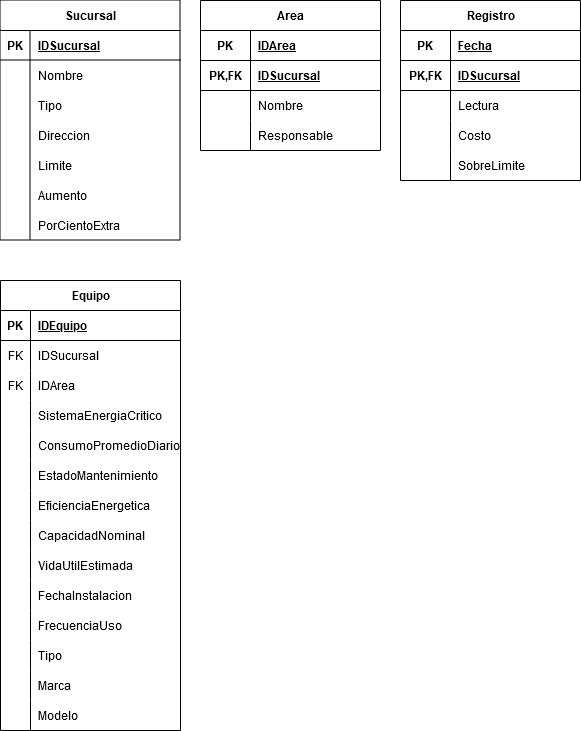
\includegraphics[scale=0.5]{Imagenes/Informe1/EsquemaRelacional.png}
\caption{Descomposición del esquema relacional de la base de datos modelado a través de tablas.}
\label{esquemaRelacional}
\end{figure}


\subsection{De la correctitud del diseño de la Base de Datos}
Recordemos que un diseño es teóricamente correcto si se encuentra en 3FN o superior y cumple las propiedades PPDF y PLJ.

El esquema relacional que se presentó en la sección anterior se encuentra en 3FN y cumple la PPDF como resultado de aplicar el algoritmo
de 3FN. Sin embargo no se comprobó si cumple la PLJ, por tanto no se puede afirmar que sea un diseño teóricamente correcto.

Se podría lograr el cumplimiento de la PLJ aplicando el lema de Ullman, lo cual se dejó pendiente para futuras revisiones del modelo de la
base de datos.

\newpage
\listoffigures

\end{document}